\chapter{Automatic Text Summarization}
\thispagestyle{fancy}
\label{chap:Automatic Text Summarization}

\noindent
Unter Kenntnis der theoretischen Grundlagen werden die Ausführungen zur \ac{ATS} in diesem Kapitel ausgeweitet, basierend auf den einordnenden Worten aus der Einleitung. Dabei werden die grundlegenden Informationen zusammengefasst und mithilfe des neu gewonnenen Wissens nochmalig eingeordnet. Darüber hinaus werden insbesondere der Forschungsstand vertieft und vergleichbare Arbeiten analysiert, nun auch technisch.\\

\noindent
Es ist bekannt, dass...
- Typen der Zusammenfassung (Tabelle von Gambhir S.5), entsprechende Daten notwendig
- Text mit S.2 meiner Arbeit verschriften
- Technische Aspekte von S.2 aufgreifen, bspw. m < n, bei jedem Typ gültig, mehr Mathematik aus Papern einbinden
- Ziel nennen und somit ATS-Typ eingrenzen
- Forschungsstand, der den ATS-Typ betrifft, vorstellen, bspw. BERT/ BART aufgreifen/ kritisieren
- Ansätze vergleichbarer Arbeiten genauer vorstellen, S. 4-5, teilweise von dort auch Text übernehmen
- Verwendung von BERT, XLM-R und BART dokumentieren, Nicht-Verwendung von ELMo und GPT entsprechend
- Kontext: Was hat man bereits in NLP gemacht? Was ist SOTA? Was mache ich?

\noindent
Die in dieser Arbeit konzipierte Architektur ist als Sequence-to-Sequence-Transformer-Modell zu verstehen. Dabei wird sowohl der Encoder als auch der Decoder durch ein eigenständiges gemäß \ac{TL} vortrainiertes Modell repräsentiert. Aufgrund der bereits beschriebenen Grundlagen wird nun die weitergehende Konfiguration der Architektur definiert. Hierbei gibt es unter anderem die folgenden beiden Möglichkeiten, um den Encoder zum \ac{NLU} und den Decoder zur \ac{NLG} zu initialisieren \cite[S.~2]{ROT20}.\\

\noindent
Einerseits ist es möglich, den Encoder und den Decoder jeweils mit einem autarken Modell zu initialisieren, beispielsweise den Encoder mit \ac{BERT} und den Decoder mit \ac{GPT}. Andererseits ist es aber auch möglich, sowohl den Encoder als auch den Decoder mit dem gleichen Checkpoint eines Modells zu initialisieren, welches ursprünglich nur als Encoder trainiert wurde, beispielsweise mit \ac{BERT}. Gemäß \ac{TL} wird so im Kontext von \ac{NLP} und \ac{ATS} das Neuerlernen einer Sprache umgangen. Aufgrund der Verfügbarkeit von \ac{BERT} wird in der Folge nur letztere Möglichkeit betrachtet. Die folgenden Ausführungen sind in \autoref{pic:EncoderDecoderBert} visualisiert \cite[S.~2-3]{ROT20}.\\

\begin{figure}[h!]
  \centering
  \fbox{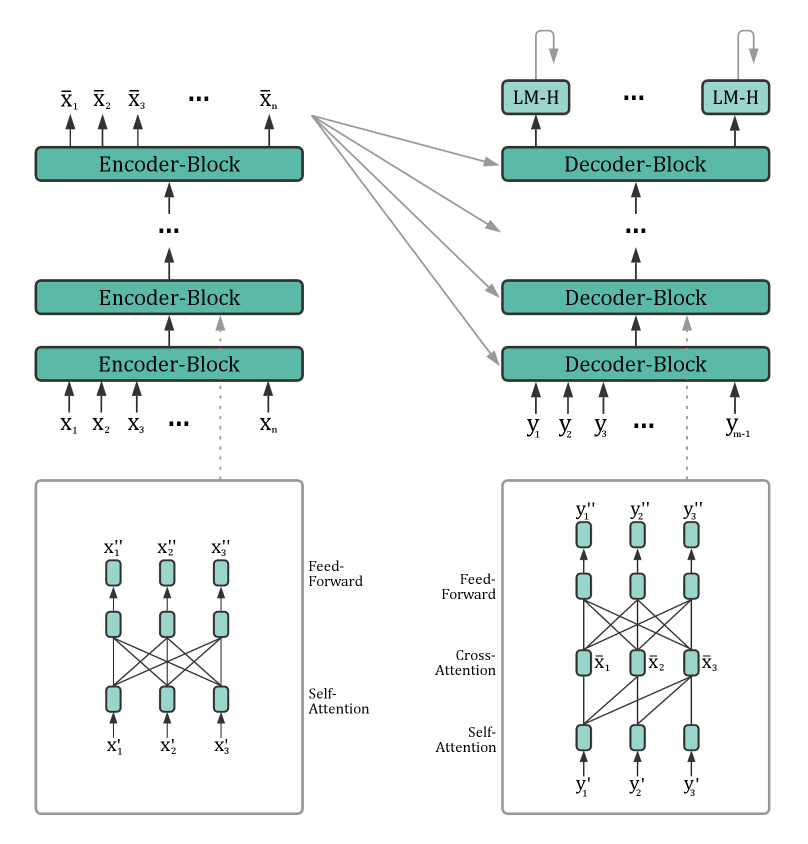
\includegraphics[width=0.8\linewidth]{./source/images/encoderdecoderbert.png}}
  \caption{Sequence-to-Sequence-Transformer-Modell mit BERT \cite{VON20}.}
  \label{pic:EncoderDecoderBert}
\end{figure}

\noindent
Die Gewichte der bidirektionalen Self-Attention-Schichten und der Feed-Forward-Schichten aller Encoder-Blöcke werden mit den vortrainierten Gewichten von \ac{BERT} initialisiert. Dabei kann der Encoder schlichtweg als \ac{BERT} in seiner Reinform verstanden werden. Der Decoder hingegen bedarf mindestens der nachstehenden Anpassungen \cite{VON20}.\\

\noindent
Zunächst werden sogenannte Cross-Attention-Schichten zwischen den Self-Attention-Schichten und den Feed-Forward-Schichten aller \ac{BERT}-Blöcke eingeführt, um die kontextbasierten Sequenzen verarbeiten zu können. Die Gewichte der Cross-Attention-Schichten werden hierbei zufällig initialisiert \cite{VON20}.\\

\noindent
Zudem werden die bidirektionalen Self-Attention-Schichten zu unidirektionalen Self-Attention-Schichten transformiert, um der autoregressiven Funktionsweise eines Decoders gerecht zu werden. Bei der autoregressiven \ac{NLG} wird angenommen, dass die Wahrscheinlichkeitsverteilung einer Sequenz in das Produkt der bedingten nächsten Wortverteilungen zerlegt werden kann \cite{VON20}. Beide Attention-Schichten basieren auf den gleichen Projektionen aus Key, Query und Value, weshalb die Gewichte dieser Schichten weiterhin mit den Werten von \ac{BERT} initialisiert werden können. Die unidirektionalen Self-Attention-Schichten berücksichtigen nun nur noch vorangegangene Token, nicht mehr auch die nachstehenden Token. Dies führt zu veränderten Ausgabevektoren im Vergleich zum ursprünglich \ac{BERT}, obwohl sie die gleichen Gewichte teilen \cite[S.~2]{ROT20}.\\

\noindent
Zuletzt wird dem Decoder eine sogenannte Language-Model-Head-Schicht hinzugefügt, dessen Gewichte mit denen des gewählten Word Embeddings initialisiert werden. Hierbei handelt es sich erneut um \ac{BERT}. Es wird deutlich, dass sich der Encoder und der Decoder viele Gewichte teilen können. Dies führt zu einer erheblichen Reduktion des Speicherbedarfs, während die Qualität anschließender \ac{NLP}-Aufgaben nahezu unverändert bleibt \cite[S.~2]{ROT20}.\\

\noindent
Die Textinhalte der Datengrundlage bedürfen überdies keiner weitergehenden Vorverarbeitung im herkömmlichen Sinne. Diese ist bekanntermaßen sehr individuell und stark modellabhängig. Unter Verwendung der als sehr robust geltenden Transformer-Architekturen entfällt daher die sonst übliche Textbereinigung sowie die Textnormalisierung. Dies unterliegt der Annahme, dass Transformer-Architekturen potenziell aus jeder Eigenart ein relevantes Feature schaffen können, welches das spätere Ergebnis begünstigt. Von der zugeführten Interpunktion und den vielfältigen Wortformen wird sich indes erhofft, potenzielle Mehr- oder Uneindeutigkeiten zu minimieren. Das Fine-Tuning sollte darüber hinaus stets unter gleichen Bedingungen wie das initiale Training stattfinden. Gleichzeitig sinkt hierdurch der vorverarbeitende Aufwand und damit auch etwaige Wartezeiten bei der praktischen Anwendung bereits trainierter Modelle in Echtzeit. Dennoch ist es möglich, bestimmte Vorverarbeitungsschritte a posteriori zu implementieren. Die Auswirkungen auf das Modell und die entsprechenden Ergebnisse würden somit zugleich messbar.\\

\noindent
In der sonstigen technischen Vorbereitung ist weiterhin ein Tokenizer zu definieren. Dieser entstammt ebenfalls \ac{BERT} und berücksichtigt Groß- und Kleinschreibung. \ac{BERT} kann Sequenzen bis zu einer maximalen Länge von 512 Token verarbeiten. Dies unterschreitet zwar die durchschnittliche Textlänge der beschriebenen Korpora, kann jedoch unter der Annahme, dass wichtige Informationen zumeist am Anfang von Texten stehen, akzeptiert werden \cite{VON20}.\\

\noindent
Von einer schlichten Erhöhung der maximalen Tokenlänge ist indes abzuraten, da hierbei ein quadratischer Anstieg der Rechenzeit und des Speicherbedarfs zu erwarten ist. Zudem wurde \ac{BERT} ausschließlich auf Texten mit einer maximalen Tokenlänge von 512 trainiert. Ein denkbarer Lösungsansatz, welcher an dieser Stelle nur genannt sei, ist der sogenannte Sliding-Window-Approach. Hierbei besteht jedoch die Gefahr, dass langfristige Abhängigkeiten verloren gehen. Zuvor sind außerdem entsprechende Testläufe durchzuführen. Weiterhin existieren Ansätze wie etwa Longformer oder auch Big Bird, welche die Verarbeitung langer Sequenzen verfolgen \cite{ZAH21}. Diese versuchen zugleich, lineare Komplexität zu erreichen, beispielsweise mithilfe lokaler Attention-Mechanismen, die wiederum mit globaler Attention verknüpft sind \cite{BEL20}. Ein eher anwendungsbezogener Workaround besteht hingegen darin, den jeweils eingehenden Rohtext alle 512 Token zu unterteilen, die Subtexte einzeln zusammenzufassen und die Zusammenfassungen zu konkatenieren. Dies betrifft jedoch nicht das eigentliche Training \cite[S.~2]{DIN20}.\\

\noindent
Texte werden also zusammenfassend in den nachfolgenden Schritten jeweils nach 512 Token abgeschnitten. Die maximale Tokenlänge der entstehenden Zusammenfassungen wird auf 128 limitiert. Anpassungen, welche etwa im Laufe der experimentgetriebenen Entwicklung und Optimierung an Potenzial gewinnen, werden an den entsprechenden Stellen ergründet und evaluiert.
